\documentclass[9pt, a4paper, twocolumn]{article}

% Packages
\usepackage[margin=1.3cm, top=1.6cm, bottom=1.4cm, columnsep=0.5cm]{geometry}
\usepackage{graphicx}
\usepackage{booktabs}
\usepackage{array}
\usepackage{tabularx}
\usepackage{hyperref}
\usepackage{enumitem}
\usepackage{parskip}
\usepackage{titlesec}
\usepackage{xcolor}
\usepackage{fancyhdr}
\usepackage{microtype}
\usepackage{lmodern}
\usepackage[T1]{fontenc}
\usepackage{tikz}
\usetikzlibrary{shapes.geometric, arrows.meta, positioning, fit, backgrounds, calc}

% Colors
\definecolor{indigo}{RGB}{79, 70, 229}
\definecolor{indigolite}{RGB}{224, 231, 255}
\definecolor{slate}{RGB}{71, 85, 105}
\definecolor{emerald}{RGB}{16, 185, 129}
\definecolor{amber}{RGB}{245, 158, 11}
\definecolor{rose}{RGB}{244, 63, 94}
\definecolor{sky}{RGB}{14, 165, 233}
\definecolor{lightgray}{RGB}{241, 245, 249}

% Section formatting
\titleformat{\section}{\small\bfseries\color{indigo}}{}{0em}{}[\vspace{-2pt}\color{indigo}\rule{\linewidth}{0.5pt}]
\titleformat{\subsection}{\footnotesize\bfseries\color{slate}}{}{0em}{}
\titlespacing{\section}{0pt}{8pt}{3pt}
\titlespacing{\subsection}{0pt}{5pt}{2pt}

% Header / Footer
\pagestyle{fancy}
\fancyhf{}
\rhead{\tiny\color{slate} InsightEngine, April 2026}
\lhead{\tiny\color{slate} Prototyping Products with Data and AI}
\cfoot{\tiny\thepage}
\renewcommand{\headrulewidth}{0.3pt}

\hypersetup{colorlinks=true, linkcolor=indigo, urlcolor=indigo}

\setlength{\parskip}{3pt}
\setlength{\parindent}{0pt}

% ─────────────────────────────────────────────
\begin{document}

% Full-width title block
\twocolumn[{%
\begin{center}
  {\large\bfseries\color{indigo} InsightEngine}\\[2pt]
  {\normalsize\color{slate} Building a Market Intelligence Platform, Start to Finish}\\[4pt]
  {\small Prototyping Products with Data and Artificial Intelligence \quad\textbullet\quad April 2026}
\end{center}
\vspace{2pt}
\noindent\rule{\linewidth}{0.8pt}
\vspace{2pt}
\begin{center}
\begin{minipage}{0.90\linewidth}
\footnotesize\itshape\color{slate}
This is the story of InsightEngine: a market intelligence platform we built over a semester that turns raw customer reviews, stock prices, and news signals into audience-specific competitive dashboards. The idea started simple. The execution did not. This post documents the journey honestly---what worked, what we threw away, and what we learned about building with LLMs under real constraints.
\end{minipage}
\end{center}
\vspace{6pt}
}]

% ─── SECTION 1 ───────────────────────────────
\section{The Problem We Wanted to Solve}

The question that started everything was almost embarrassingly basic: why does competitive analysis still take weeks? The raw material---millions of customer reviews, news headlines, earnings reports---is sitting in public view. The reasoning capacity to synthesise it exists in modern language models. The bottleneck, we decided, was not data or compute. It was \textit{framing}.

A stock analyst evaluating HubSpot and a product manager at a competing CRM look at the same review corpus but need completely different things. The analyst wants sentiment trajectory and share-of-voice signals over time. The product manager wants a ranked list of the features customers complain about most. A buyer choosing between tools needs a clean value-for-money comparison. Most BI tools are built for one of these audiences and serve the other two poorly. We wanted to serve all three from a single data run.

The first sketch had three boxes on a whiteboard: \textit{scrape reviews}, \textit{score with LLM}, \textit{show chart}. It took about one afternoon of actual implementation for the diagram to become considerably more complex.

% ─── SECTION 2 ───────────────────────────────
\section{What We Built}

InsightEngine is a web application where a user logs in, picks an audience (Investor, Company, or Customer) and one of twelve industry verticals---CRM, food delivery, ride-sharing, SaaS collaboration, e-commerce, restaurants, hospitality, banking, healthcare, travel, telecom, and insurance---then sees a dashboard of charts and AI-generated insights tailored to that combination. The same underlying data produces three entirely different views depending on who is asking.

The platform covers between three and six competing companies per industry, scored across five to eight competitive dimensions, producing a normalised score matrix that drives all the visualisations. Before reaching the dashboard, users pass through a short onboarding chat where they describe their role and what they are trying to understand. The LLM extracts structured preferences from that conversation and surfaces a personalised insight section above the standard analysis.

On the technical side, a React frontend talks to a FastAPI backend over a REST and SSE API. The backend pulls review data from up to four sources, scores each review individually with a language model, synthesises insights in a single generation call, then enriches the result with live stock prices, news headlines, and Glassdoor ratings. The whole pipeline runs in under thirty seconds on Groq's free tier.

\vspace{3pt}
{\fontsize{7.5pt}{9.5pt}\selectfont
\begin{tabularx}{\linewidth}{@{}l X@{}}
\toprule
\textbf{Layer} & \textbf{Technology} \\
\midrule
Frontend  & React 18, Vite 6, TypeScript, Tailwind CSS v4, Recharts \\
Backend   & Python 3.9, FastAPI, Uvicorn \\
Database  & SQLite via SQLAlchemy (auth, saved views, chat history) \\
LLM       & Groq (\texttt{llama-3.3-70b}) or OpenAI, user-selectable \\
Reviews   & Apify (G2, Capterra), SerpAPI Google Maps, Kaggle datasets \\
Market    & Alpha Vantage (stock quotes), SerpAPI (News, Trends, Glassdoor) \\
Auth      & JWT via python-jose, bcrypt password hashing \\
\bottomrule
\end{tabularx}
}
\vspace{3pt}

\begin{figure}[h]
\centering
\resizebox{0.7\linewidth}{!}{%
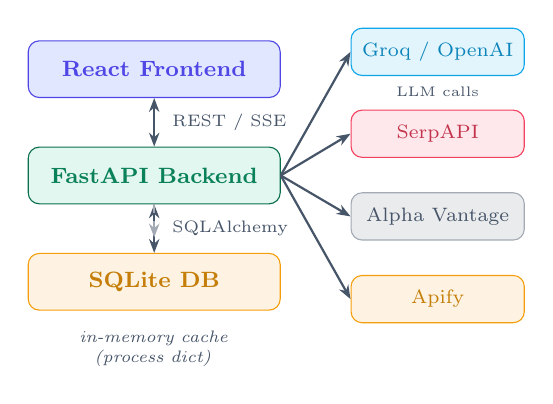
\begin{tikzpicture}[x=1cm, y=1cm,
  lay/.style={rectangle, rounded corners=4pt,
    font=\fontsize{8pt}{9pt}\selectfont\bfseries,
    minimum width=3.2cm, minimum height=0.72cm,
    text centered, inner sep=4pt},
  ext/.style={rectangle, rounded corners=4pt,
    font=\fontsize{7pt}{8pt}\selectfont,
    minimum width=2.2cm, minimum height=0.6cm,
    text centered, inner sep=3pt},
  arr/.style={-{Stealth[length=5pt]}, thick, color=slate},
  barr/.style={{Stealth[length=5pt]}-{Stealth[length=5pt]}, thick, color=slate}
]
% Main vertical stack
\node[lay, fill=indigolite, draw=indigo, text=indigo]
  at (1.6, 0) (fe) {React Frontend};
\node[lay, fill=emerald!12, draw=emerald!60!black, text=emerald!70!black]
  at (1.6,-1.35) (be) {FastAPI Backend};
\node[lay, fill=amber!12, draw=amber, text=amber!80!black]
  at (1.6,-2.7) (db) {SQLite DB};
% Bidirectional arrows in stack
\draw[barr] (fe.south) -- (be.north)
  node[midway, right=0.1cm, font=\fontsize{6pt}{7pt}\selectfont\color{slate}] {REST / SSE};
\draw[barr] (be.south) -- (db.north)
  node[midway, right=0.1cm, font=\fontsize{6pt}{7pt}\selectfont\color{slate}] {SQLAlchemy};
% External APIs on the right
\node[ext, fill=sky!12, draw=sky, text=sky!80!black]
  at (5.2,  0.22) (groq) {Groq / OpenAI};
\node[ext, fill=rose!12, draw=rose, text=rose!80!black]
  at (5.2, -0.82) (serp) {SerpAPI};
\node[ext, fill=slate!12, draw=slate!50, text=slate]
  at (5.2, -1.87) (av)   {Alpha Vantage};
\node[ext, fill=amber!12, draw=amber, text=amber!80!black]
  at (5.2, -2.92) (apify){Apify};
% Arrows from backend to external APIs
\draw[arr] (be.east) -- (groq.west);
\node[font=\fontsize{5.5pt}{6.5pt}\selectfont\color{slate}, below=0.01cm of groq] {LLM calls};
\draw[arr] (be.east) -- (serp.west);
\draw[arr] (be.east) -- (av.west);
\draw[arr] (be.east) -- (apify.west);
% In-memory cache annotation
\node[font=\fontsize{6pt}{7pt}\selectfont\color{slate},
      align=center, text width=2.4cm]
  at (1.6,-3.55) {\textit{in-memory cache\\(process dict)}};
\draw[arr, dashed, color=slate!50] (be.south) -- ++(0,-0.42);
\end{tikzpicture}%
}
\caption{\footnotesize High-level architecture. The React frontend communicates with FastAPI over REST and SSE. The backend calls external APIs for LLM inference, market data, and review scraping, and persists auth data in SQLite.}
\label{fig:sysarch}
\end{figure}

% ─── SECTION 3 ───────────────────────────────
\section{How the Architecture Actually Came Together}

The three-box whiteboard diagram became a four-stage pipeline fairly quickly. The \textbf{Fetch} stage sources reviews in priority order---Kaggle datasets first (largest and most structured for supported industries), then SerpAPI Google Maps for restaurant and hospitality verticals, then Apify's managed scrapers for G2 and Capterra, and finally a local JSON file as a final fallback that is always available. The \textbf{Score} stage submits each review to a fast language model---\texttt{llama-3.1-8b-instant}---with a structured prompt, running up to eight reviews concurrently. The \textbf{Insights} stage sends the full score matrix and a selection of representative excerpts to a larger model---\texttt{llama-3.3-70b-versatile}---in a single synthesis call, getting back both a JSON array of tagged insights and a short \textit{executive brief}: a plain-prose paragraph that orients the reader before they encounter individual insight cards. The \textbf{Enrich} stage fetches live signals independently: stock price history, PE and PEG ratios, news headlines, Google Trends share-of-voice, and Glassdoor ratings.

\begin{figure}[htbp]
\centering
\resizebox{\linewidth}{!}{%
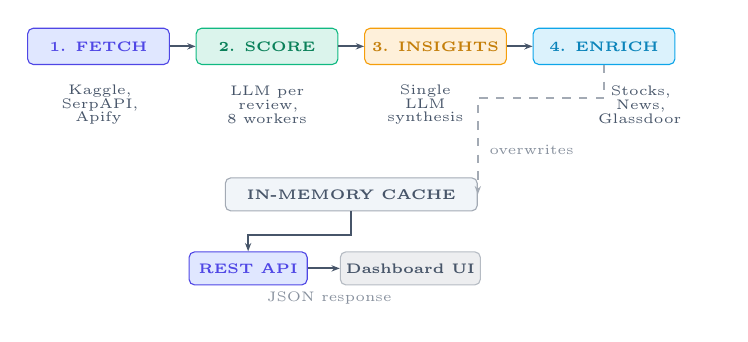
\begin{tikzpicture}[x=1cm, y=1cm,
  trim left=-0.9cm,
  sbox/.style={rectangle, rounded corners=2pt,
    minimum width=1.8cm, minimum height=0.46cm,
    font=\fontsize{5pt}{6pt}\selectfont\bfseries,
    text centered, inner sep=2pt},
  wbox/.style={rectangle, rounded corners=2pt,
    minimum width=1.7cm, minimum height=0.42cm,
    font=\fontsize{5pt}{6pt}\selectfont\bfseries,
    text centered, inner sep=2pt},
  arr/.style={-{Stealth[length=3pt]}, thick, color=slate},
  darr/.style={-{Stealth[length=3pt]}, thick, color=slate!50, dashed},
  lbl/.style={font=\fontsize{4pt}{5pt}\selectfont\color{slate},
    align=center, text width=1.8cm}
]
\node[sbox, fill=indigolite, draw=indigo, text=indigo]            at (0,    0) (fetch)  {1. FETCH};
\node[sbox, fill=emerald!15, draw=emerald, text=emerald!70!black] at (2.14, 0) (score)  {2. SCORE};
\node[sbox, fill=amber!15,   draw=amber,   text=amber!80!black]   at (4.28, 0) (ins)    {3. INSIGHTS};
\node[sbox, fill=sky!15,     draw=sky,     text=sky!80!black]     at (6.42, 0) (enrich) {4. ENRICH};
\draw[arr] (fetch.east) -- (score.west);
\draw[arr] (score.east) -- (ins.west);
\draw[arr] (ins.east)   -- (enrich.west);
\node[lbl] at (0,    -0.74) {Kaggle,\\SerpAPI,\\Apify};
\node[lbl] at (2.14, -0.74) {LLM per\\review,\\8 workers};
\node[lbl] at (4.15, -0.74) {Single\\LLM\\synthesis};
\node[lbl] at (6.87, -0.74) {Stocks,\\News,\\Glassdoor};
\node[wbox, fill=lightgray, draw=slate!50, text=slate,
      minimum width=3.2cm] at (3.21, -1.88) (cache) {IN-MEMORY CACHE};
\draw[darr] (enrich.south) -- ++(0,-0.42) -| (cache.east);
\node[font=\fontsize{3.6pt}{4.4pt}\selectfont\color{slate!65}] at (5.5, -1.31) {overwrites};
\node[wbox, fill=indigolite, draw=indigo, text=indigo,
      minimum width=1.5cm] at (1.9,  -2.82) (api) {REST API};
\node[wbox, fill=slate!10, draw=slate!40, text=slate,
      minimum width=1.5cm] at (3.96, -2.82) (ui)  {Dashboard UI};
\draw[arr] (cache.south) -- ++(0,-0.30) -| (api.north);
\draw[arr] (api.east) -- (ui.west);
\node[font=\fontsize{3.6pt}{4.4pt}\selectfont\color{slate!65}] at (2.93, -3.2) {JSON response};
\end{tikzpicture}%
}
\caption{\footnotesize Four-stage SSE pipeline. Each stage emits a progress event to the frontend. Results overwrite the in-memory cache and serve all subsequent page loads.}
\label{fig:pipeline}
\end{figure}

One architectural decision that shaped everything else was running a single pipeline and fanning out the results to three audience views rather than running three separate pipelines. The practical reason was simple: Groq's free tier has token-per-minute limits, and tripling the number of synthesis calls would have pushed a full analysis run close to four minutes while risking rate limit errors. Collapsing to one pipeline forced us to design the insight generation prompt so the LLM tags each insight with an audience label---Investors, Companies, or Customers---at generation time. The frontend then applies a second gate via a \texttt{CHARTS\_BY\_AUDIENCE} map, ensuring each tab renders only the charts and data cards relevant to that stakeholder type. What started as a cost optimisation became the platform's most distinctive feature.

The audience routing model ended up looking like Figure~\ref{fig:audience}. Each tab sees a completely different set of charts: investors get stock performance history with five-year price charts, PE and PEG ratios, news headlines, sentiment trends, and share-of-voice; companies get the radar chart, a full dimension heatmap, score deltas versus the category benchmark, and Glassdoor employee ratings; customers get a head-to-head comparison table with the per-dimension winner highlighted, AI-matched recommendation cards by buyer profile, and a positioning map of price versus perceived value.

\begin{figure}[h]
\centering
\resizebox{0.9\linewidth}{!}{
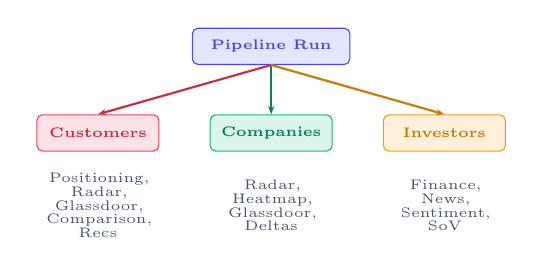
\begin{tikzpicture}[x=1cm, y=1cm,
  pbox/.style={rectangle, rounded corners=2pt,
    font=\fontsize{5pt}{6pt}\selectfont\bfseries,
    minimum width=1.55cm, minimum height=0.46cm,
    text centered, inner sep=2pt},
  arr/.style={-{Stealth[length=3pt]}, thick},
  lbl/.style={font=\fontsize{4pt}{5pt}\selectfont\color{slate},
    align=center, text width=1.55cm}
]
\node[pbox, fill=indigolite, draw=indigo, text=indigo,
      minimum width=2.0cm] at (2.6, 0) (pipe) {Pipeline Run};

\node[pbox, fill=rose!15,    draw=rose,    text=rose!80!black]
  at (0.4,  -1.1) (cust) {Customers};
\node[pbox, fill=emerald!15, draw=emerald, text=emerald!70!black]
  at (2.6,  -1.1) (comp) {Companies};
\node[pbox, fill=amber!15,   draw=amber,   text=amber!80!black]
  at (4.8,  -1.1) (inv)  {Investors};

\draw[arr, color=rose!80!black]    (pipe.south) -- (cust.north);
\draw[arr, color=emerald!70!black] (pipe.south) -- (comp.north);
\draw[arr, color=amber!80!black]   (pipe.south) -- (inv.north);

\node[lbl] at (0.4,  -2.02) {Positioning,\\Radar, Glassdoor,\\Comparison, Recs};
\node[lbl] at (2.6,  -2.02) {Radar,\\Heatmap,\\Glassdoor, Deltas};
\node[lbl] at (4.8,  -2.02) {Finance,\\News,\\Sentiment, SoV};
\end{tikzpicture}
}
\caption{\footnotesize One pipeline run fans out to three independent views, each with its own chart set and insight bucket.}
\label{fig:audience}
\end{figure}

% ─── SECTION 4 ───────────────────────────────
\section{The Parts That Took the Most Time}

\subsection{Getting the LLM to Score Consistently}

Scoring reviews with a language model sounds straightforward until you actually do it. Each review is submitted to \texttt{llama-3.1-8b-instant} with a prompt defining the task, the list of competitive dimensions, and an instruction to return a JSON object with one integer score per dimension from 0 to 100. The model should return null for dimensions not mentioned in the review.

In practice, early versions of the prompt produced a mean score of 71 across all dimensions. Every company looked good and the comparative signal was buried in a narrow band at the top of the range. The model was not lying---71 is a plausible reading of most customer reviews, which tend toward the positive unless something went seriously wrong. The problem was that a compressed scale is useless for comparison. We tried lowering the anchor, rewording the task, and adding explicit boundary examples. What finally worked was specifying in the prompt that a score of 50 represents a genuinely mixed or neutral experience, and that scores below 40 should be reserved for reviews that describe concrete failures. Adding those anchors pushed the distribution into a range where differences between companies were actually visible.

The same synthesis call that produces the insight array also generates the executive brief---a two to three sentence paragraph in plain prose that summarises the key competitive dynamic for the current audience. This was added after early user testing: without it, readers would land on a list of individual insight cards with no orienting context. The brief is togglable so returning users can skip it.

\begin{figure}[h]
\centering
\resizebox{\linewidth}{!}{%
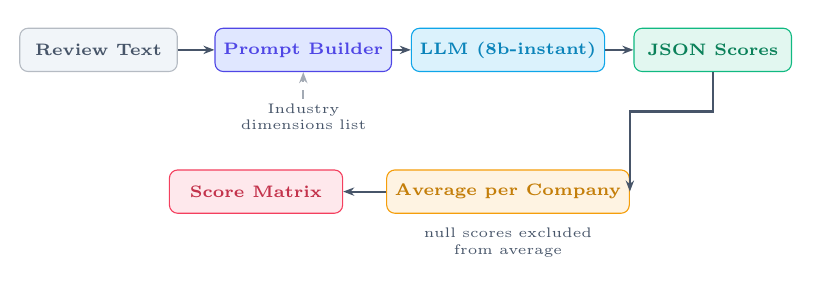
\begin{tikzpicture}[x=1cm, y=1cm,
  trim left=-0.9cm,
  bx/.style={rectangle, rounded corners=3pt,
    font=\fontsize{6pt}{7pt}\selectfont\bfseries,
    minimum width=2.0cm, minimum height=0.55cm,
    text centered, inner sep=3pt},
  arr/.style={-{Stealth[length=4pt]}, thick, color=slate},
  lbl/.style={font=\fontsize{5pt}{6pt}\selectfont\color{slate}, align=center}
]
\node[bx, fill=lightgray, draw=slate!40, text=slate]
  at (0,   0) (rev)    {Review Text};
\node[bx, fill=indigolite, draw=indigo, text=indigo]
  at (2.6, 0) (prompt) {Prompt Builder};
\node[bx, fill=sky!15, draw=sky, text=sky!80!black]
  at (5.2, 0) (llm)    {LLM (8b-instant)};
\node[bx, fill=emerald!12, draw=emerald, text=emerald!70!black]
  at (7.8, 0) (json)   {JSON Scores};
\draw[arr] (rev.east)    -- (prompt.west);
\draw[arr] (prompt.east) -- (llm.west);
\draw[arr] (llm.east)    -- (json.west);
\node[lbl, text width=1.8cm] at (2.6, -0.85) {Industry\\dimensions list};
\draw[arr, dashed, color=slate!50] (2.6,-0.62) -- (prompt.south);
\node[bx, fill=amber!12, draw=amber, text=amber!80!black,
      minimum width=2.6cm] at (5.2, -1.8) (agg) {Average per Company};
\node[bx, fill=rose!12, draw=rose, text=rose!80!black,
      minimum width=2.2cm] at (2.0, -1.8) (matrix) {Score Matrix};
\draw[arr] (json.south) -- ++(0,-0.5) -| (agg.east);
\draw[arr] (agg.west) -- (matrix.east);
\node[lbl, text width=2.4cm] at (5.2, -2.45) {null scores excluded\\from average};
\end{tikzpicture}%
}
\caption{\footnotesize Per-review LLM scoring flow. Up to eight reviews run concurrently. Dimensions not mentioned in a review return null and are excluded from the per-company average.}
\label{fig:scoring}
\end{figure}

\subsection{Scraping turned out not to be one thing}

What the whiteboard diagram called ``scrape reviews'' became four separate data paths. G2 and Capterra require a managed scraper that handles login walls and pagination---we used Apify for that. Google Maps reviews have a completely different structure and are more representative than software review platforms for restaurants and hospitality, so SerpAPI's Maps endpoint handles those. For food delivery and ride-sharing, Kaggle hosts pre-built datasets that are richer than anything we could scrape live. And beneath all of that sits a set of local JSON files with sample reviews that always work regardless of which API keys are present.

Wrapping all of this in a graceful fallback chain---try Kaggle, then SerpAPI, then Apify, then local file---was one of the cleaner decisions we made. The \texttt{resources/adapters.py} file acts as a central dispatcher that catches import errors and missing keys and returns \texttt{None} rather than crashing. The calling code checks for \texttt{None} before including a field in the API response, and the frontend renders a card only when the corresponding data field is non-null. The platform demos at any point in development because the pipeline degrades gracefully instead of failing visibly.

% ─── SECTION 5 ───────────────────────────────
\section{What We Threw Away}

The first version of the codebase ran three separate analysis pipelines, one per audience. It felt natural to model it that way. It was also a disaster: total run time crept past four minutes, Groq rate limits became unreliable, and the three synthesis prompts produced subtly inconsistent framing. Collapsing to a single pipeline with audience fan-out cut run time by roughly 60\% and produced a design that was actually better---one where the insight routing decision is made by the LLM during generation rather than by keyword matching after the fact.

The original frontend was a single scrollable page with all charts visible and an audience dropdown. On a real screen this was overwhelming: a radar chart, a competitive heatmap, a stock chart, and a news feed all loaded simultaneously with no clear reading order. Switching to a tabbed interface with one tab per audience took half a day of work and made the product noticeably more convincing in a demo context. URL routing was retained so that each tab has its own bookmarkable address.

We also planned to use the OpenWebNinja Glassdoor API for employee ratings. The key was added to the environment file and we tried to connect to the endpoint, but the API returned an AWS API Gateway ``Missing Authentication Token'' response regardless of what path we attempted, and the documentation was too sparse to debug systematically. Rather than spend days on a third-party API with no clear path forward, we pivoted to extracting ratings from Google Search snippets via SerpAPI---a targeted \texttt{site:glassdoor.com} search whose results are parsed with a regular expression. It works about 70\% of the time, which was acceptable under time constraints.

An earlier version of the Investors tab included a customer migration flow visualisation, showing movement between competitors based on hash-derived values. During review we realised that entirely synthetic data presented in a chart format gives the impression of real analytical validity, when in fact it had none. We removed it rather than leave something misleading in the product.

% ─── SECTION 6 ───────────────────────────────
\section{What We Learned About Building with AI}

Claude Code was the primary coding assistant throughout. For tasks with clear specifications---the SSE streaming loop, the SQLAlchemy models, the JWT auth flow, the Recharts visualisation components---AI-generated code was correct on the first attempt and needed only minor adjustments. For tasks requiring accumulated project context, such as the audience routing logic or the cache fallback strategy, the AI needed explicit framing before it could produce something architecturally coherent. The adapter pattern in \texttt{resources/adapters.py}---nested \texttt{try/except ImportError} blocks around every optional dependency---was suggested by Claude Code when we asked how to make optional packages safe. We would have arrived at something similar, but the AI applied it consistently across all adapters immediately, which saved time and produced a more uniform codebase.

LLM prompts required more iteration than we expected. Initial drafts for both the review scoring and the insight synthesis prompts went through roughly ten rounds of refinement before the outputs were consistent enough to trust. AI-assisted prompt engineering---generating a sample output, identifying a failure mode, asking the model to suggest a fix---reduced the number of manual iterations considerably.

Several bugs were diagnosed with AI help. The most significant was a race condition in the chat streaming endpoint where a database session was being shared across concurrent SSE events, leading to intermittent SQLAlchemy errors. The fix---moving session creation inside the generator function---was identified correctly from the error message alone. A second bug was a \texttt{NoneType} division error when the LLM returned null for a dimension used in a positioning calculation. The fix was a one-line change suggested immediately upon showing the traceback.

AI assistance had real limits. For anything requiring understanding of \textit{why} a specific workaround was in place---a quirk of the SerpAPI Glassdoor extraction, or the cache invalidation order---the AI required substantial context and sometimes produced suggestions that were locally correct but architecturally misaligned. Every AI-generated code change needed human review. The AI also occasionally introduced subtle issues, such as replacing straight quotes with typographic curly quotes in source files, which caused build failures.

The broader lesson is that AI tooling changed the shape of development work more than it changed the amount. Configuration, boilerplate, and debugging took less time. Architectural decisions, prompt engineering, and verifying that generated code actually matched the design intent took at least as much as they would have without AI assistance.

% ─── SECTION 7 ───────────────────────────────
\section{Where It Landed}

The final platform covers twelve industries, scores up to 64 reviews per run across six companies in under thirty seconds, and delivers three meaningfully different dashboards from a single data pipeline. Investor and company views diverge substantially on the same underlying dataset---confirming that audience routing produces distinct signals rather than merely relabelling the same content. The live enrichment layer---real stock prices, valuation tables, news headlines, and Glassdoor ratings on the Investors tab---creates a noticeably more credible experience than a purely review-driven view.

Some constraints remain. All analysis results are lost on server restart because the cache lives in process memory rather than a database. Alpha Vantage's free tier allows 25 requests per day, and the stock chart integration now makes three calls per company (quote, monthly series, and company overview), so a single run across six publicly traded companies consumes 18 of those 25 daily requests. The SSE stream holds a Uvicorn worker thread for its full duration, which means concurrent users compete for the same thread pool---acceptable for a prototype, not for a production deployment. The OpenWebNinja Glassdoor integration was never completed; SerpAPI remains the sole source.

If we had more time, the highest-value additions would be persisting analysis results across restarts, replacing the in-process pipeline with a background task queue, and deepening the onboarding chat so it shapes not just the insight highlights but the chart selection and framing as well. The audience-routing model is the platform's most interesting axis for future development. The insight that different stakeholders need different framings of the same data seems obvious in retrospect, but it is genuinely underserved by existing tools---and it ended up being the thing that made every demo more interesting than we expected.

\vspace{5pt}
\noindent\rule{\linewidth}{0.4pt}
{\fontsize{6.5pt}{8pt}\selectfont\color{slate}
Demo account: \texttt{demo@marketlens.ai} / \texttt{demo12345}
\hfill
Source code available on request}

\end{document}
